\begin{wrapfigure}[15]{l}{0.5\textwidth}
  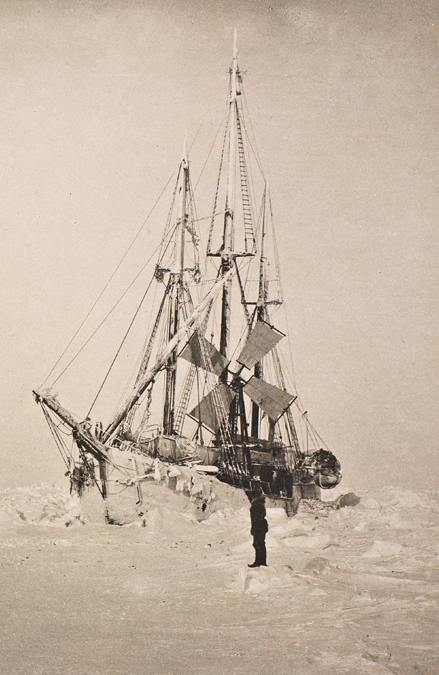
\includegraphics[scale=0.35]{Figures/Fram.jpg}
  \caption{The \emph{Fram} caught in ice in January 1895. Image courtesy of
  FramMuseum.no}
  \label{fig:Fram}
\end{wrapfigure}
The influence of the coriolis force on the currents of the ocean were first
noted by Hadley, Coriolis, and Ferrel, however the the influence of these forces
were considered to small and thereofre didn't show in the theory of the time
\cite{Ekman1905}. Ekman's adviser Bjerknes was the first to indicate the
importance of the influence of the Earth's rotation in the thoery of motions of
the ocean \cite{Ekman1905}. While the true importance of the influence of the
Coriolis force was first noted by the Norwegian scientist Fridtjof Nansen
\cite{Beesley2008, Ekman1905}. Nansen designed a vessel named, the \emph{Fram},
with the intent of allowing it to freeze in the polar ice, and in 1898 Nansen
observed the drift of the \emph{Fram} from its original location. As the vessel
drifted Nansen noticed that the drift was always $20^\circ - 40^\circ$ to the
right of the wind current \cite{Beesley2008}.

In 1905 Ekman\cite{Ekman1905} took the observations made by Nansen and developed
what is considered to be the origin of modern theories for wind-driven ocean
circulation and their effects on ocean currents \cite{Price1987}. According to
Ekman theory momentum from the wind is transferred at the surface of the ocean
to the water, as it blows accross the ocean surface, via wind stress. Then the
Earth's rotation imparts a Coriolis acceleration on the moving water which
causes a deflection of the transport to the right of the surface wind stress in
the Northern Hemisphere and to the left of the surface wind stress in the
Southern Hemisphere \cite{Beesley2008}.

The first study of wind-driven ocean circulation, where the \emph{Coriolis
parameter} varied from north to south was, introduced by Sverdrup (1947)
\cite{Fox-Kemper2003}. This variable Coriolis parameter introduced, for the
first time, an asymmetry of the problem domain by distinguishing north from
south, and thus a new term was born.  The $\nicefrac{\partial \psi}{\partial x}$
term, which involves the streamfunction, $\psi$, usually referred to as the
$\beta$-term, is an advection caused by the rotation of the Earth.

Next, Stommel (1948) combined the dynamics of \emph{western boundary currents}
with the $\beta$-term. The model developed by Stommel was a simple model which
included the $\beta$-term ($\nicefrac{\partial \psi}{\partial x}$), a bottom
friction term ($-\delta_S \nabla^2 \psi$), and a wind stress forcing term ($f$).
The resultant equation is
\begin{equation}
  \frac{\partial \psi}{\partial x} = f - \delta_s \nabla^2 \psi.
  \label{eqn:StommelModel}
\end{equation}
Stommel noted that without the $\beta$-term the solution would be symmetric in
the west-east direction and therefore no western boundary current would exist
\cite{Stommel1948}.
{\color{red} Add an overview of the progress made in creating ocean models,
including Munk, Stommel, and Charney. Maybe mention ENIAC.}

